\chapter{SYSTEM DESIGN}

\section{Technical Requirements}

\subsection{Functional Requirements}
Based on our comprehensive domain analysis \cite{automation2023}, we have identified several core functional requirements that form the foundation of the FarmBot system. The planting system serves as the primary automation component, incorporating sophisticated mechanisms for automated seed placement and spacing. This system utilizes precision robotics to ensure accurate seed deployment while maintaining optimal spacing patterns for different crop types. The tool management subsystem enables automatic switching between various implements required for different farming operations.

The irrigation control system represents another crucial functional component. It implements intelligent watering schedules based on real-time soil moisture data and environmental conditions. The system continuously monitors moisture levels through a network of sensors and adjusts watering patterns accordingly, ensuring optimal water usage while preventing both under and over-watering situations.

Our monitoring system provides comprehensive oversight of all farming operations through real-time status tracking and environmental monitoring capabilities. It collects and processes data from multiple sensor types, including temperature, humidity, light levels, and soil conditions. The growth progress tracking feature enables users to monitor plant development over time and identify potential issues early in the growing cycle.

The user interface component delivers a sophisticated yet intuitive control dashboard that makes complex farming operations accessible to users of varying technical expertise. Through this interface, users can access detailed data visualizations, manage system configurations, and monitor all aspects of their farming operations in real-time.

\subsection{Non-Functional Requirements}

The system's performance requirements establish strict criteria for operational efficiency. We mandate a maximum response time of one second for all user interface interactions to ensure smooth operation. The system must maintain 99.9% uptime to provide reliable service for critical farming operations. Additionally, the architecture supports concurrent operations, allowing multiple users to interact with the system simultaneously without performance degradation.

Reliability stands as a cornerstone of our design, with robust fault tolerance mechanisms implemented throughout the system. The data backup system maintains continuous records of all operations and sensor data, while error recovery procedures ensure minimal disruption to farming operations in case of component failures.

Usability considerations focus on making the system accessible to users with varying levels of technical expertise. The interface design follows established usability principles, incorporating responsive layouts for both desktop and mobile access. Comprehensive documentation provides users with clear guidance for all system features and operations.

\section{Behavioral Modeling}

\subsection{System Architecture Overview}
\begin{figure}[h]
    \centering
    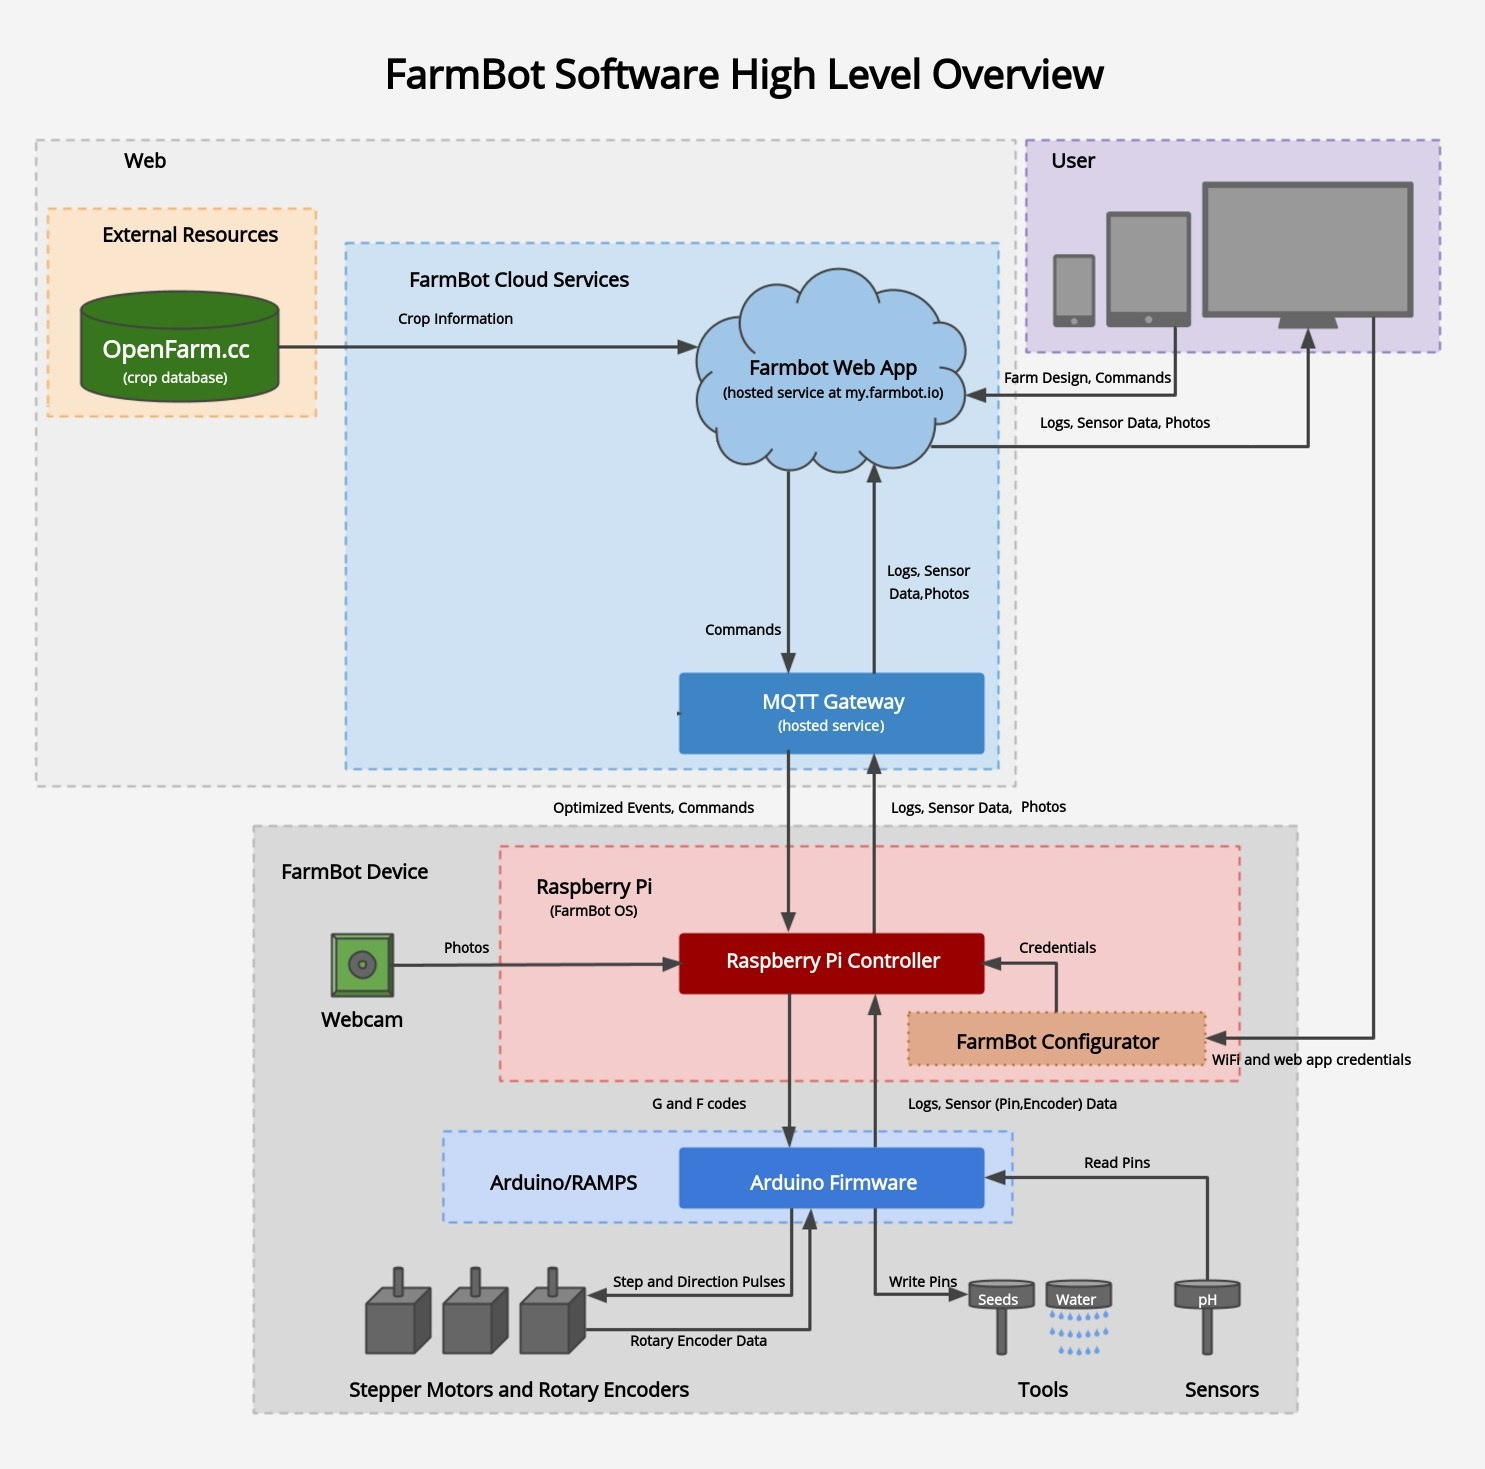
\includegraphics[width=1.0\textwidth]{img/farmbot-architecture.jpg}
    \caption{FarmBot System Architecture Overview}
    \label{fig:system-architecture}
\end{figure}

The FarmBot system architecture, as illustrated in Figure \ref{fig:system-architecture}, represents a comprehensive integration of multiple components. At the highest level, the system consists of a web-based frontend interface, cloud services for data management, and the physical FarmBot device. The architecture employs an MQTT Gateway for efficient communication between components, ensuring reliable data transfer and command execution.

\subsection{Authentication Flow}
\begin{figure}[h]
    \centering
    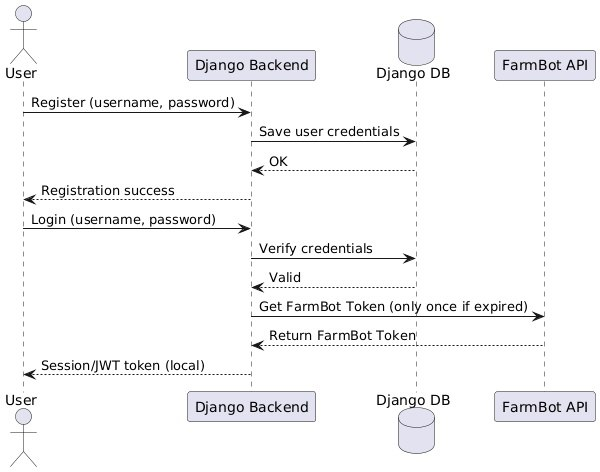
\includegraphics[width=0.8\textwidth]{img/farmbot-auth.jpg}
    \caption{FarmBot Authentication Sequence}
    \label{fig:auth-sequence}
\end{figure}

The authentication sequence shown in Figure \ref{fig:auth-sequence} demonstrates the secure user authentication process that underlies all system operations:
\begin{itemize}
    \item User registration with credential validation
    \item Secure login process with token management
    \item Session handling for maintaining secure access
    \item Integration with FarmBot API for device control
\end{itemize}

\subsection{Use Case Overview}
The system implements a comprehensive set of use cases that define the primary interactions between users and the FarmBot system. These include garden layout configuration and management, automated movement and watering operations, plant monitoring through photo capture and visualization, and system status monitoring and control. The complete use case diagram and detailed specifications can be found in Appendix A, Figure \ref{fig:usecase-detail}.

\subsection{System Operations Flow}
The system implements a sophisticated sequence of operations for handling user commands and device actions. This includes movement operations where user commands are processed through the frontend and transmitted to the FarmBot device, watering sequences with duration control and status monitoring, and photo capture operations that integrate with the onboard camera system. The detailed sequence diagram illustrating these interactions can be found in Appendix A, Figure \ref{fig:sequence-detail}.

Primary use cases:
\begin{itemize}
    \item Configure Planting Operation
    \item Manage Watering Schedule
    \item Monitor System Status
    \item Analyze Growth Data
\end{itemize}

\section{Structural Modeling}

\subsection{Component Architecture}
The FarmBot system employs a layered architecture that separates concerns while maintaining efficient communication between components. Each layer serves a specific purpose in the overall system:

\begin{itemize}
    \item Web Layer: Provides user interface and high-level control
    \item Cloud Services Layer: Manages data and coordinates operations
    \item Device Layer: Controls hardware and executes operations
    \item Sensor Layer: Collects environmental and operational data
\end{itemize}

\subsection{Hardware Integration}
The physical implementation integrates several key hardware components:

\begin{itemize}
    \item Raspberry Pi Controller: Central control unit running FarmBot OS
    \item Arduino/RAMPS Board: Hardware interface for motors and sensors
    \item Stepper Motors: Precise movement control in three axes
    \item Sensors: Environmental monitoring and position feedback
    \item Tools: Specialized implements for various farming operations
\end{itemize}

\subsection{Data Flow Architecture}
Data flows through the system following established patterns:

\begin{itemize}
    \item Command Flow: User interface → Cloud services → MQTT Gateway → Device
    \item Sensor Data: Device sensors → Arduino → Raspberry Pi → Cloud storage
    \item Status Updates: Device → MQTT Gateway → Web interface
    \item Configuration Data: Web interface → Cloud services → Device
\end{itemize}

\section{Data Management}

\subsection{Data Collection and Types}

The system collects various types of data:
\begin{itemize}
\item Images for crop/weed identification
\item Sensor readings (soil moisture, temperature, humidity)
\item Weather data
\item Soil property measurements
\end{itemize}

\subsection{Data Quality and Organization}

Data quality is maintained through:
\begin{itemize}
\item Careful sensor calibration
\item Consistent collection protocols
\item Structured storage formats (CSV, databases)
\item Comprehensive metadata
\end{itemize}

\subsection{Privacy and Ownership}

Key considerations include:
\begin{itemize}
\item Farmer control over data
\item Opt-in data sharing
\item Local data collection for site-specific conditions
\end{itemize}

\section{Visualization and Decision Support}

\subsection{Dashboard Components}

The system includes:
\begin{itemize}
\item Grid Overview
\item Photo controls
\item Bot controls
\item Bot status
\end{itemize}

\begin{figure}[H]
    \centering
    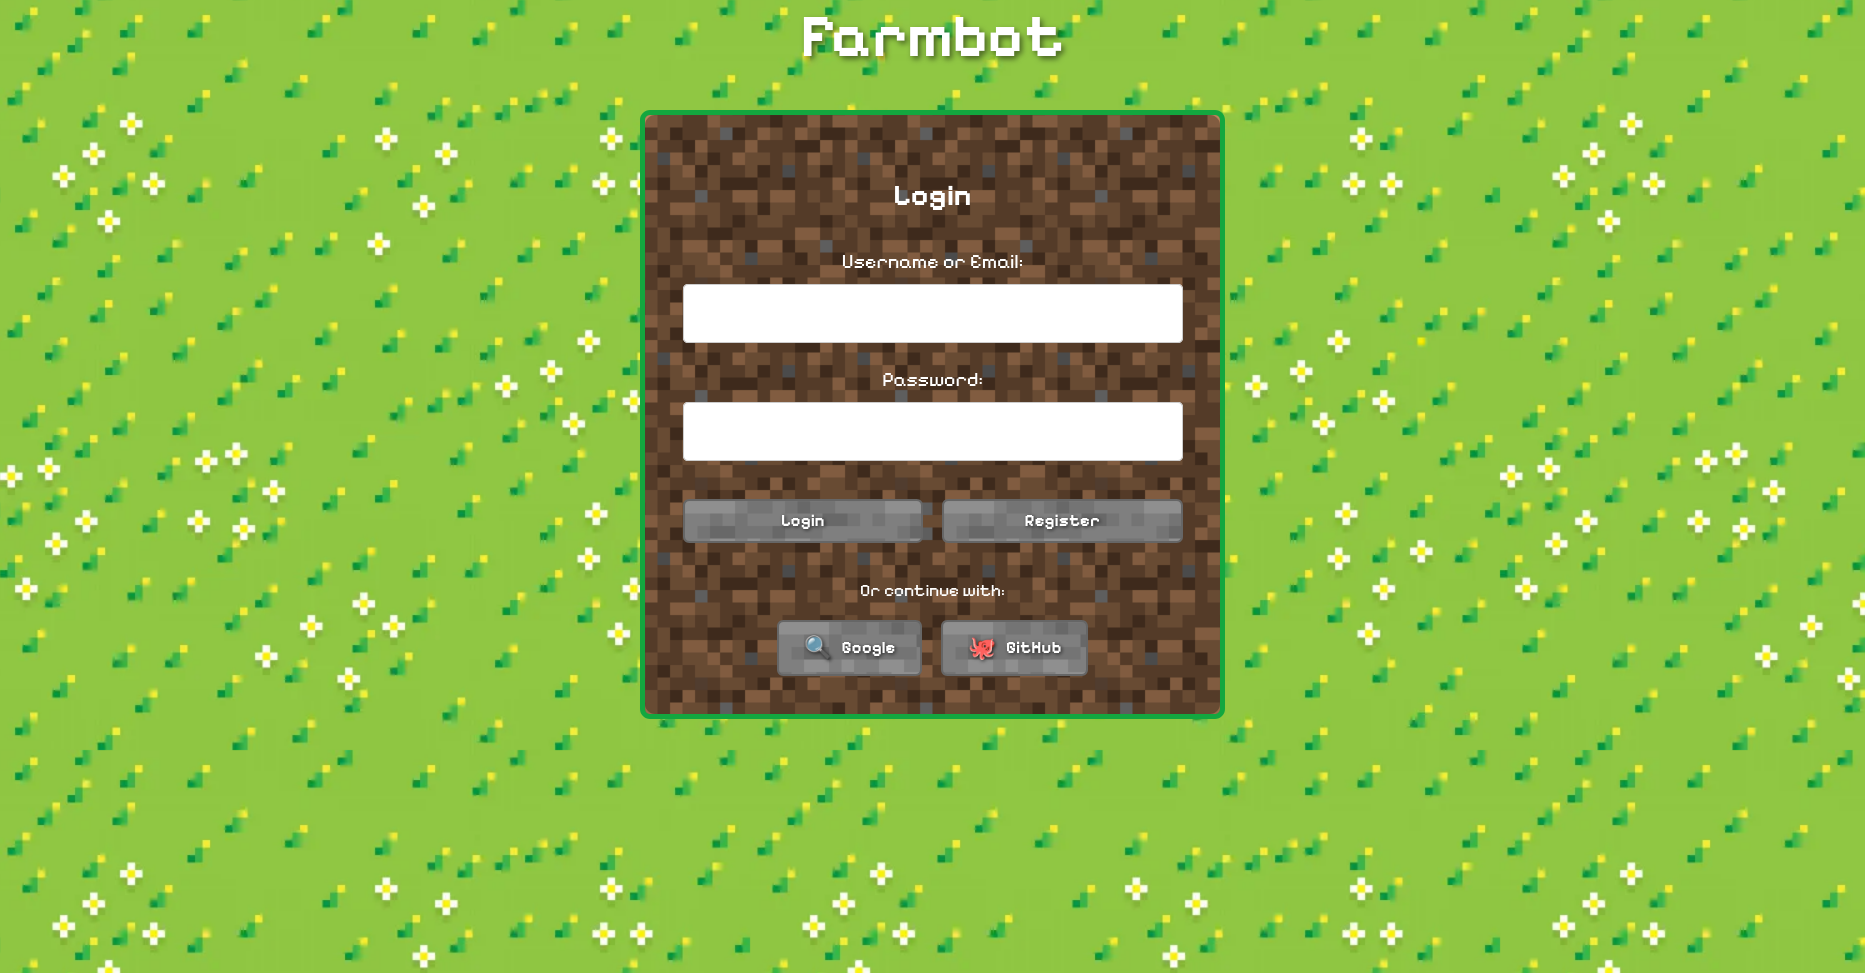
\includegraphics[width=0.8\textwidth]{img/login_page.png}
    \caption{Login Page}
    \label{fig:dashboard_login_page}
\end{figure}

\begin{figure}[H]
    \centering
    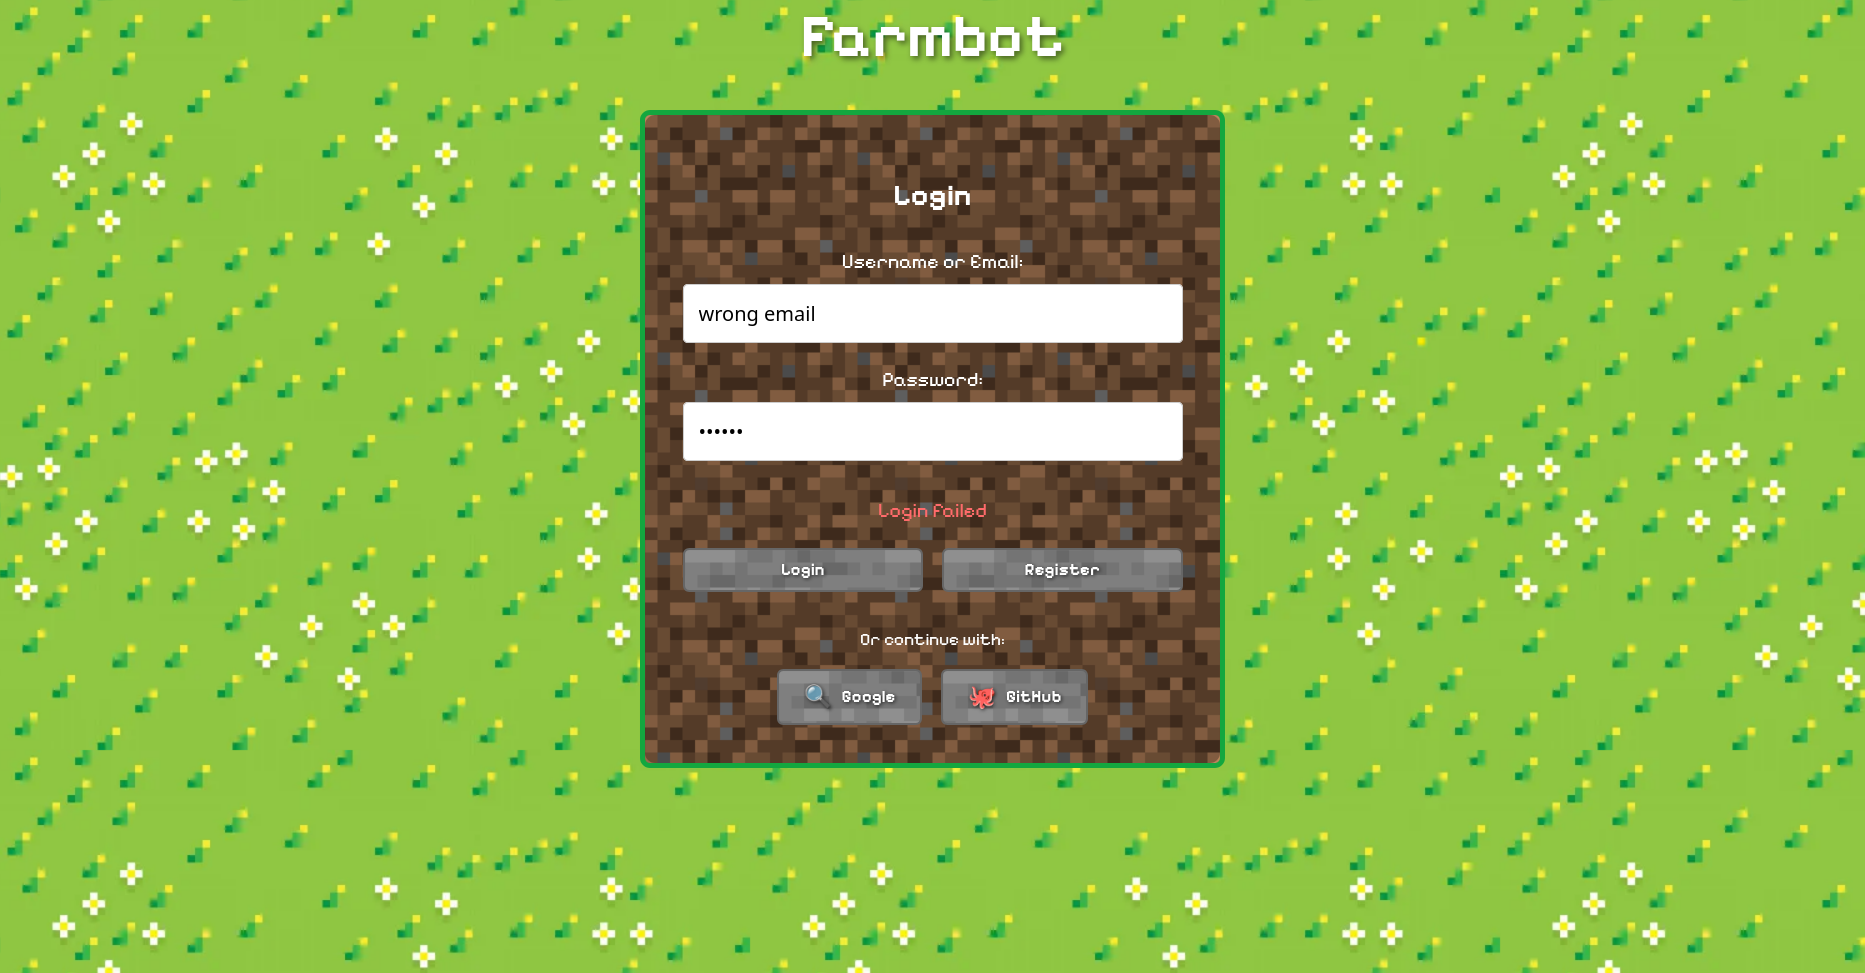
\includegraphics[width=0.8\textwidth]{img/failed_login.png}
    \caption{Failed Login}
    \label{fig:dashboard_failed_login}
\end{figure}

\begin{figure}[H]
    \centering
    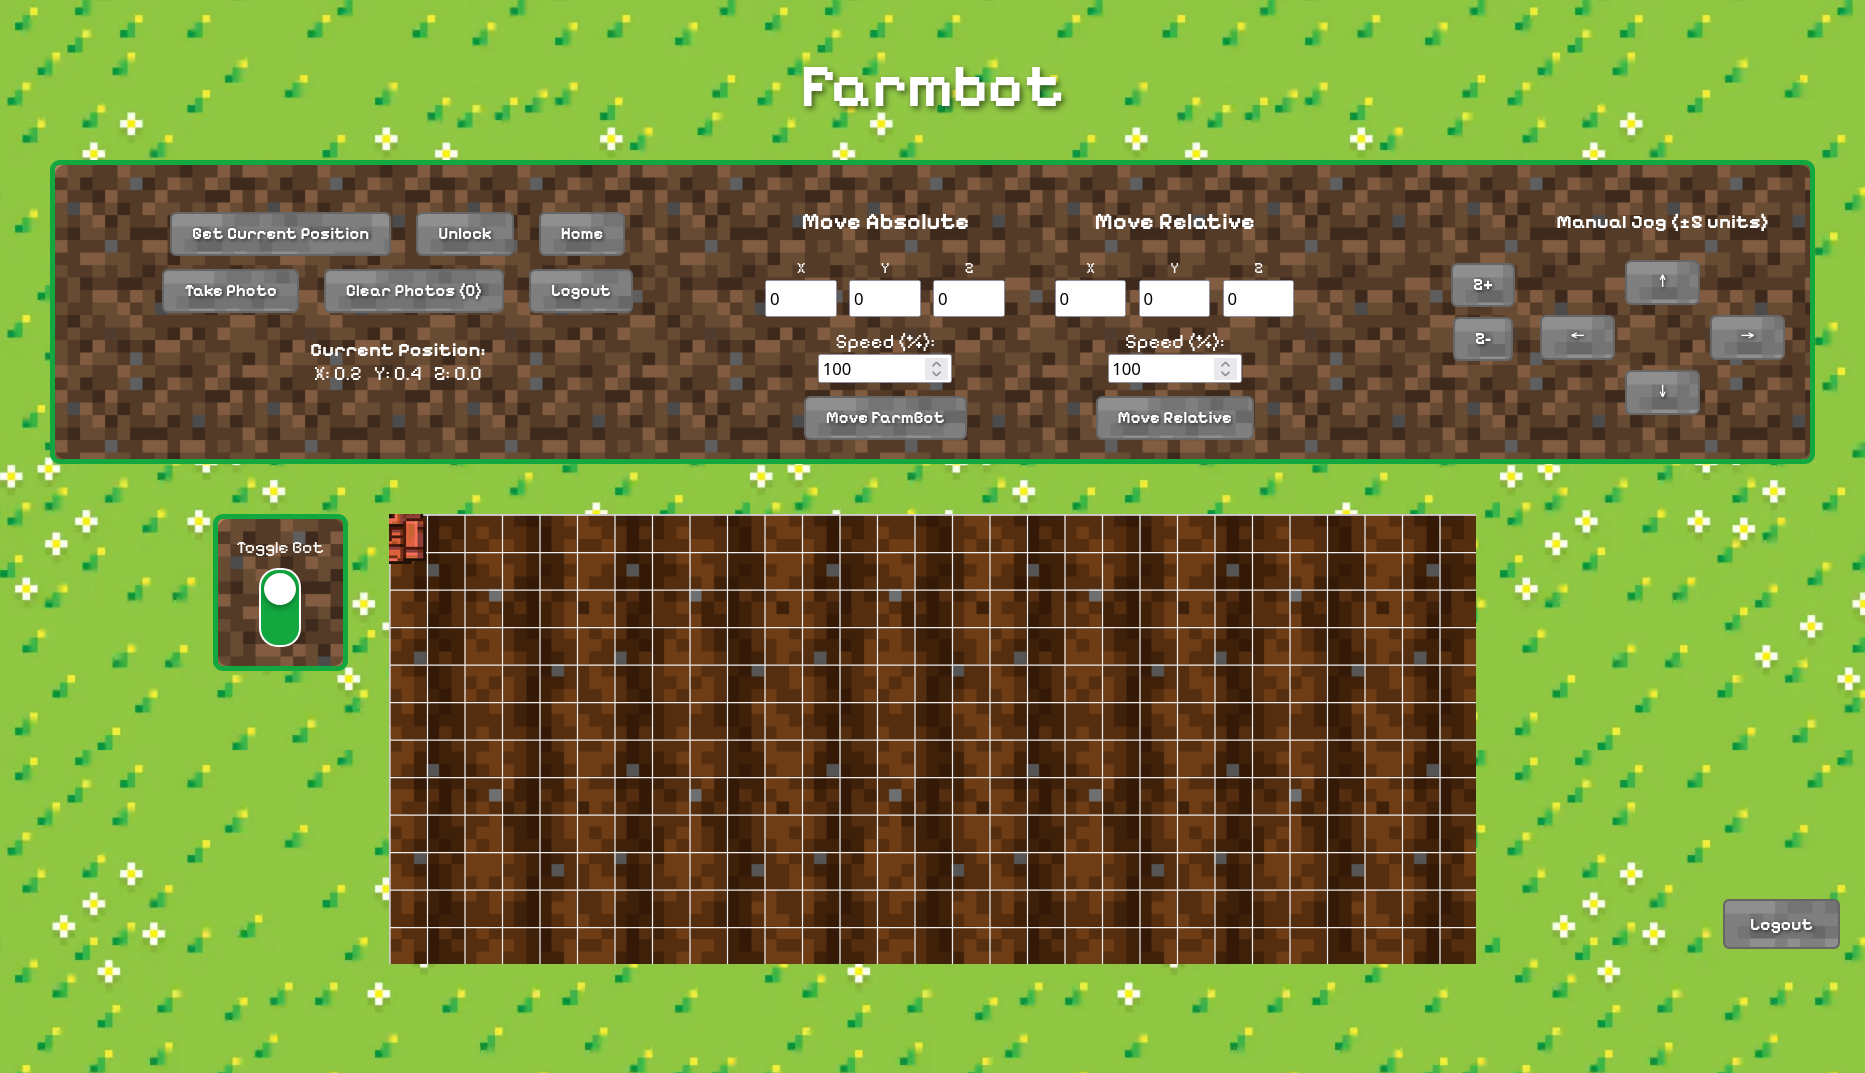
\includegraphics[width=0.8\textwidth]{img/main_page.png}
    \caption{Main Page}
    \label{fig:dashboard_main_page}
\end{figure}

\begin{figure}[H]
    \centering
    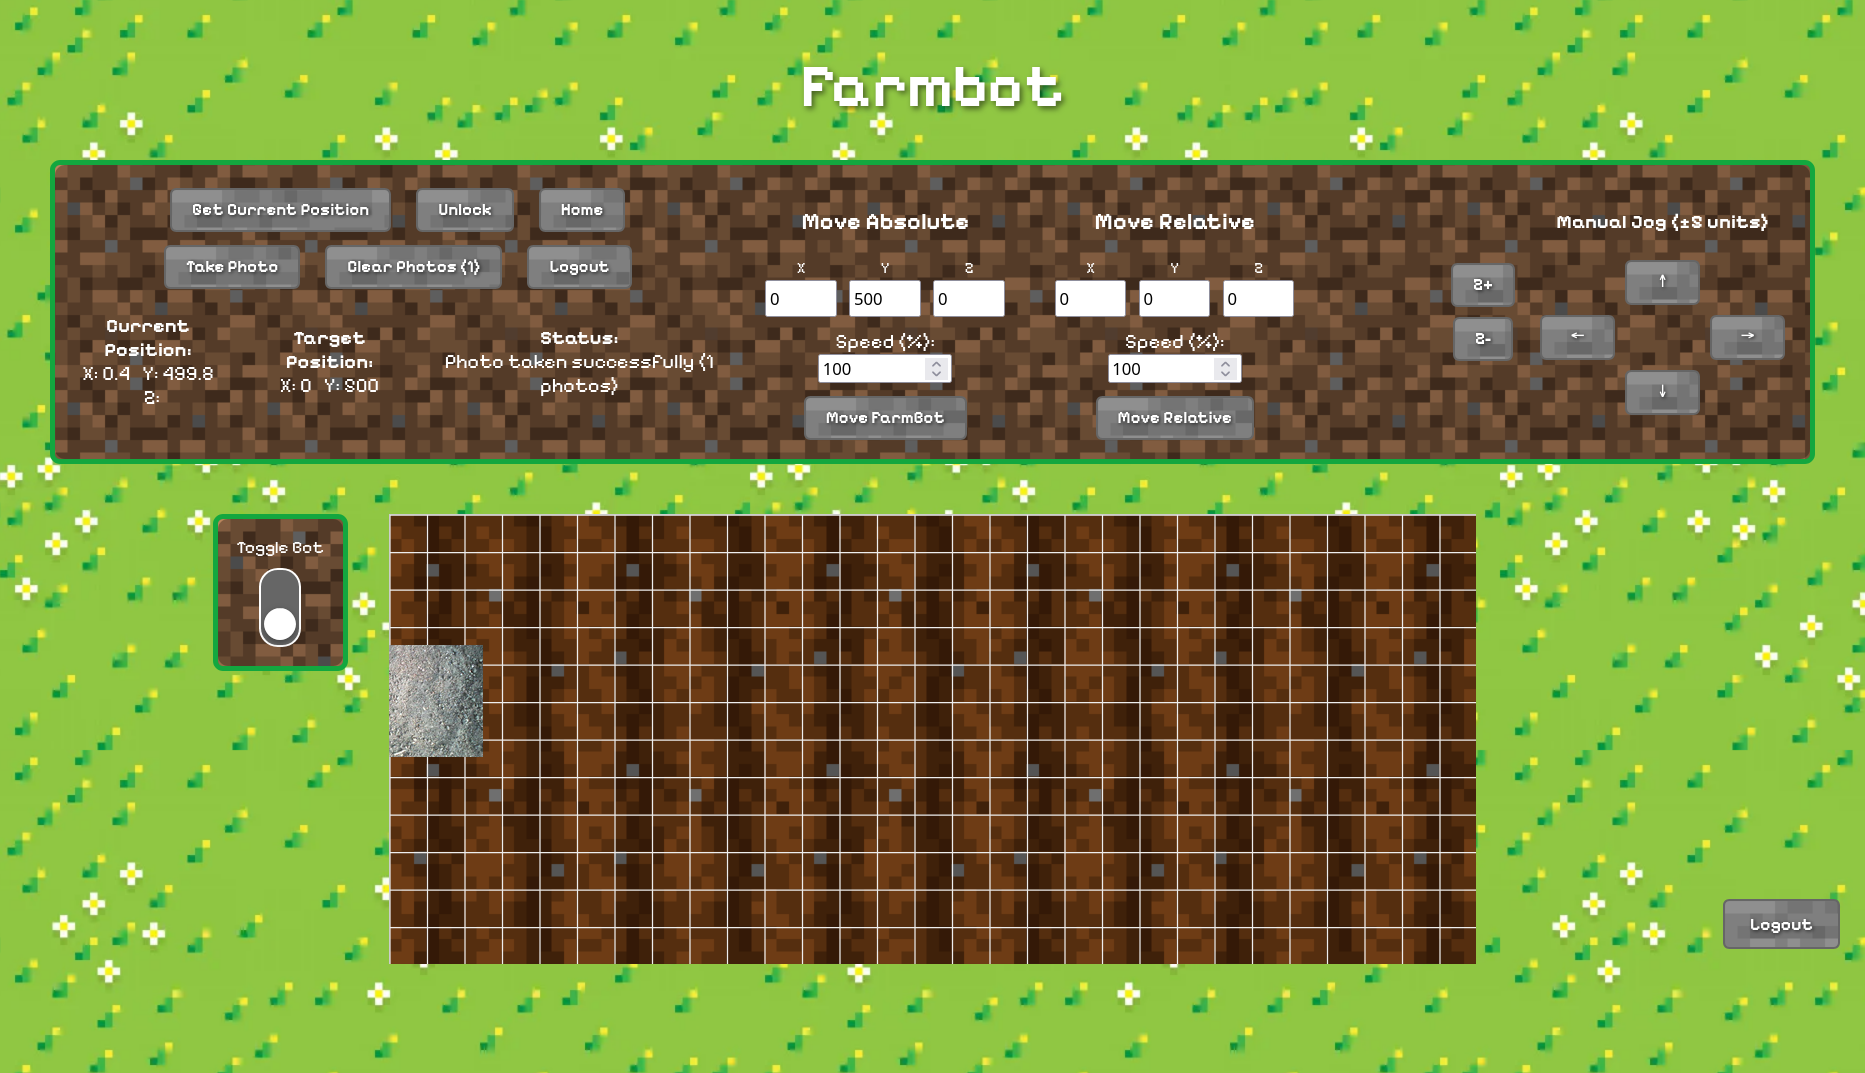
\includegraphics[width=0.8\textwidth]{img/toggling_bot_controls.png}
    \caption{Toggling Bot Controls}
    \label{fig:dashboard_toggling_bot_controls}
\end{figure}

\begin{figure}[H]
    \centering
    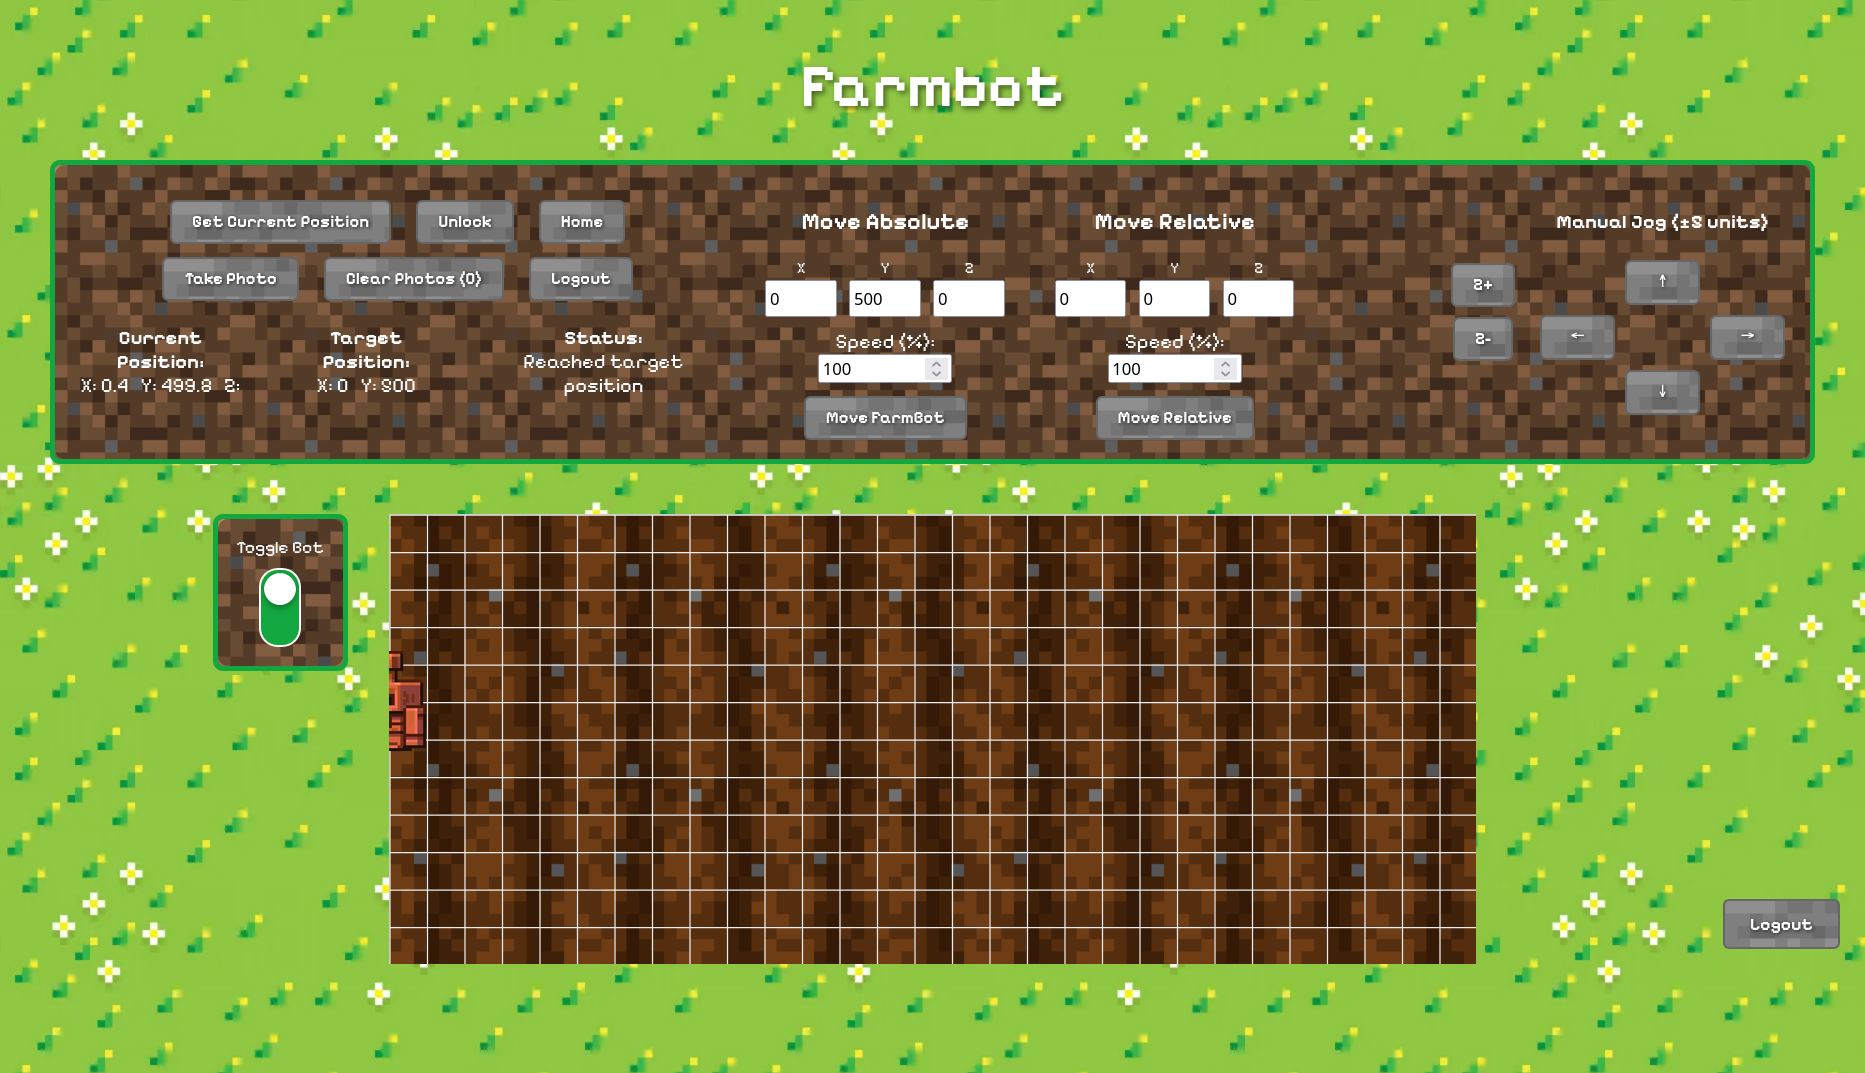
\includegraphics[width=0.8\textwidth]{img/moving_farmbot.png}
    \caption{Moving the FarmBot}
    \label{fig:dashboard_moving_farmbot}
\end{figure}

\begin{figure}[H]
    \centering
    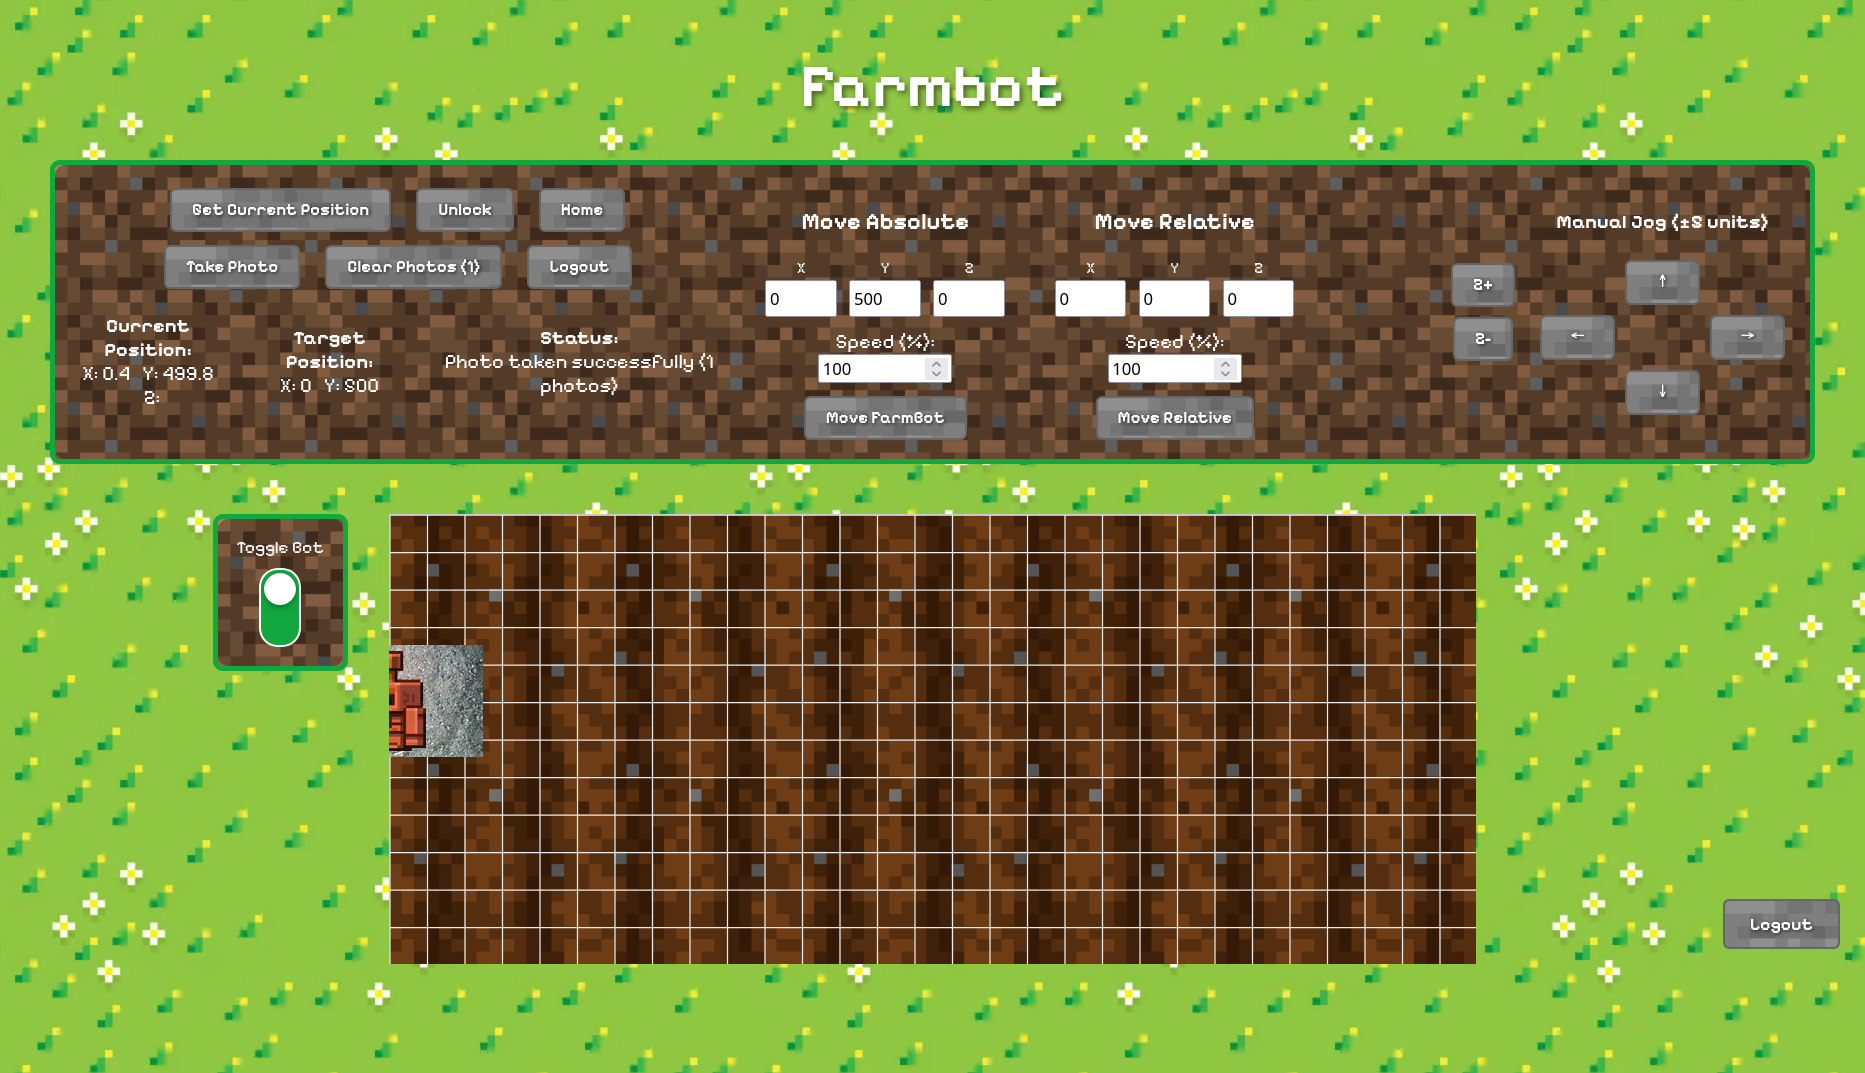
\includegraphics[width=0.8\textwidth]{img/taking_photo.png}
    \caption{Capturing Photos}
    \label{fig:dashboard_capturing_photos}
\end{figure}

\begin{figure}[H]
    \centering
    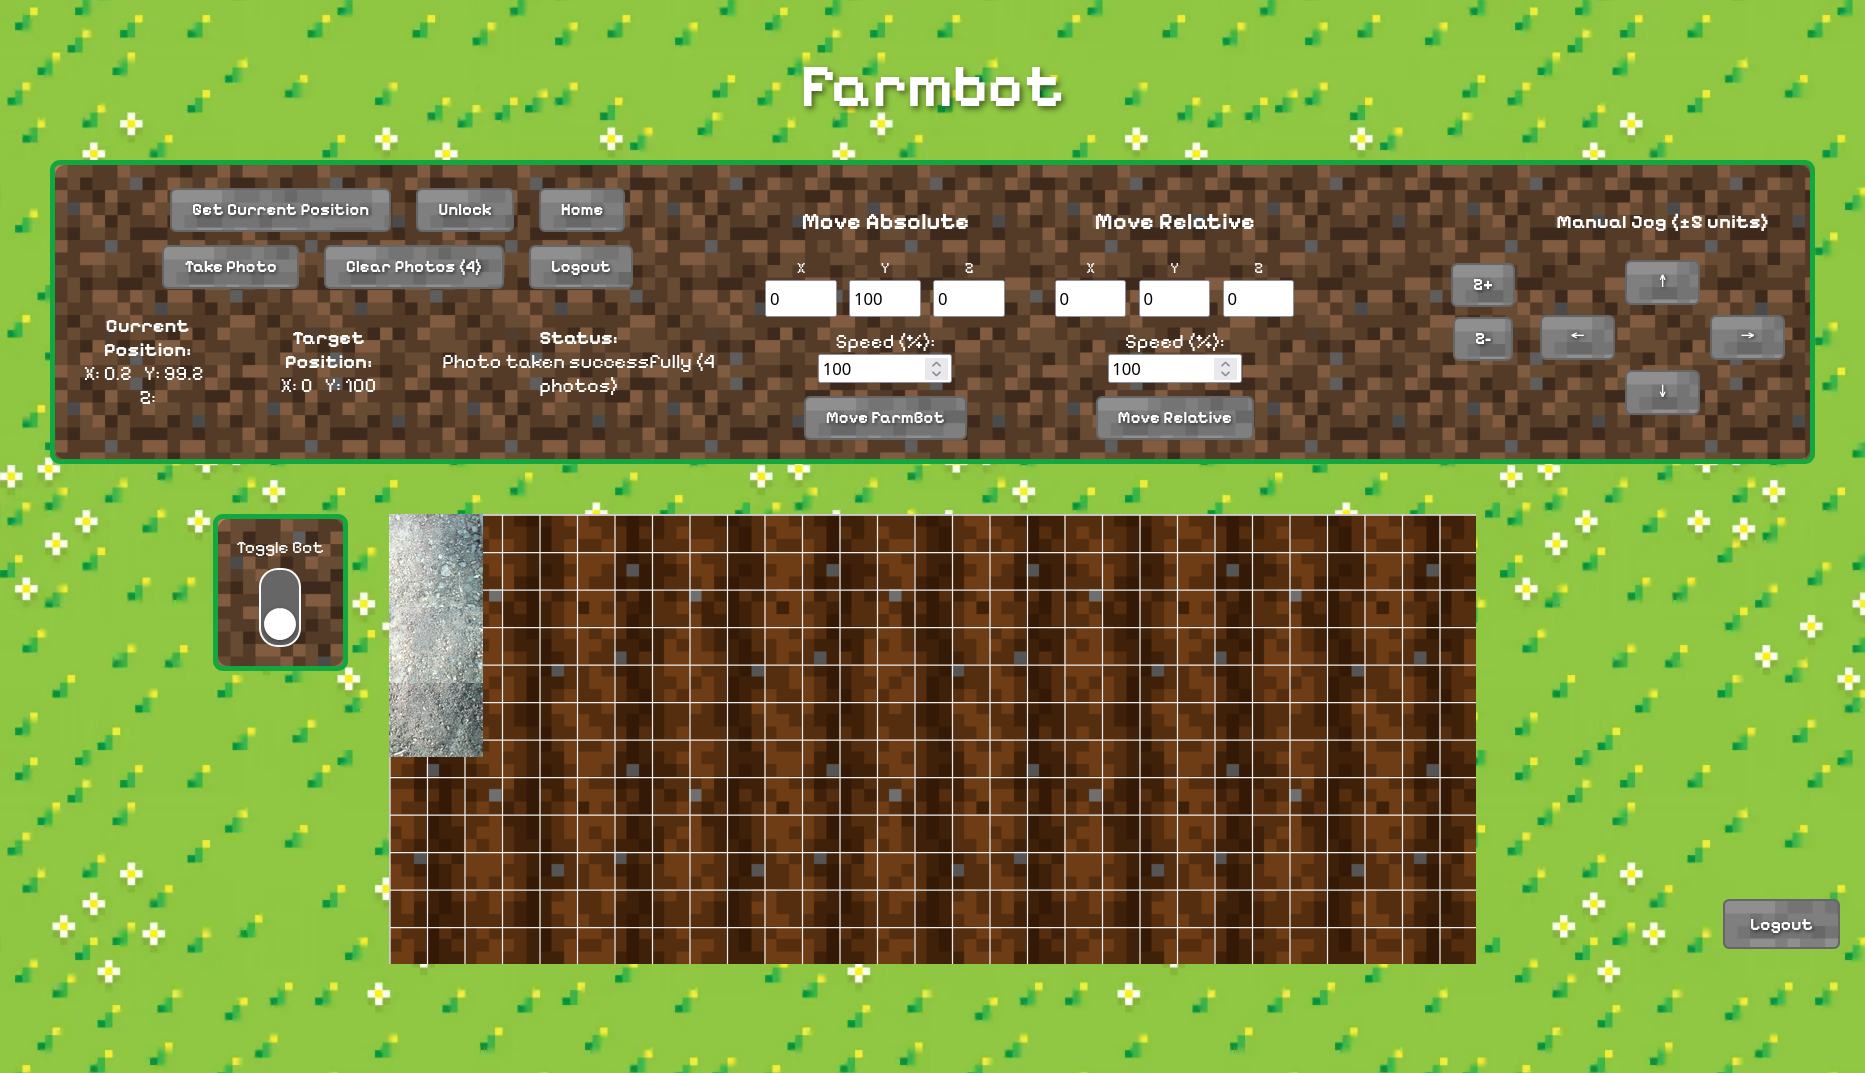
\includegraphics[width=0.8\textwidth]{img/multiple_photos.png}
    \caption{Viewing Multiple Photos}
    \label{fig:dashboard_viewing_multiple_photos}
\end{figure}

\begin{figure}[H]
    \centering
    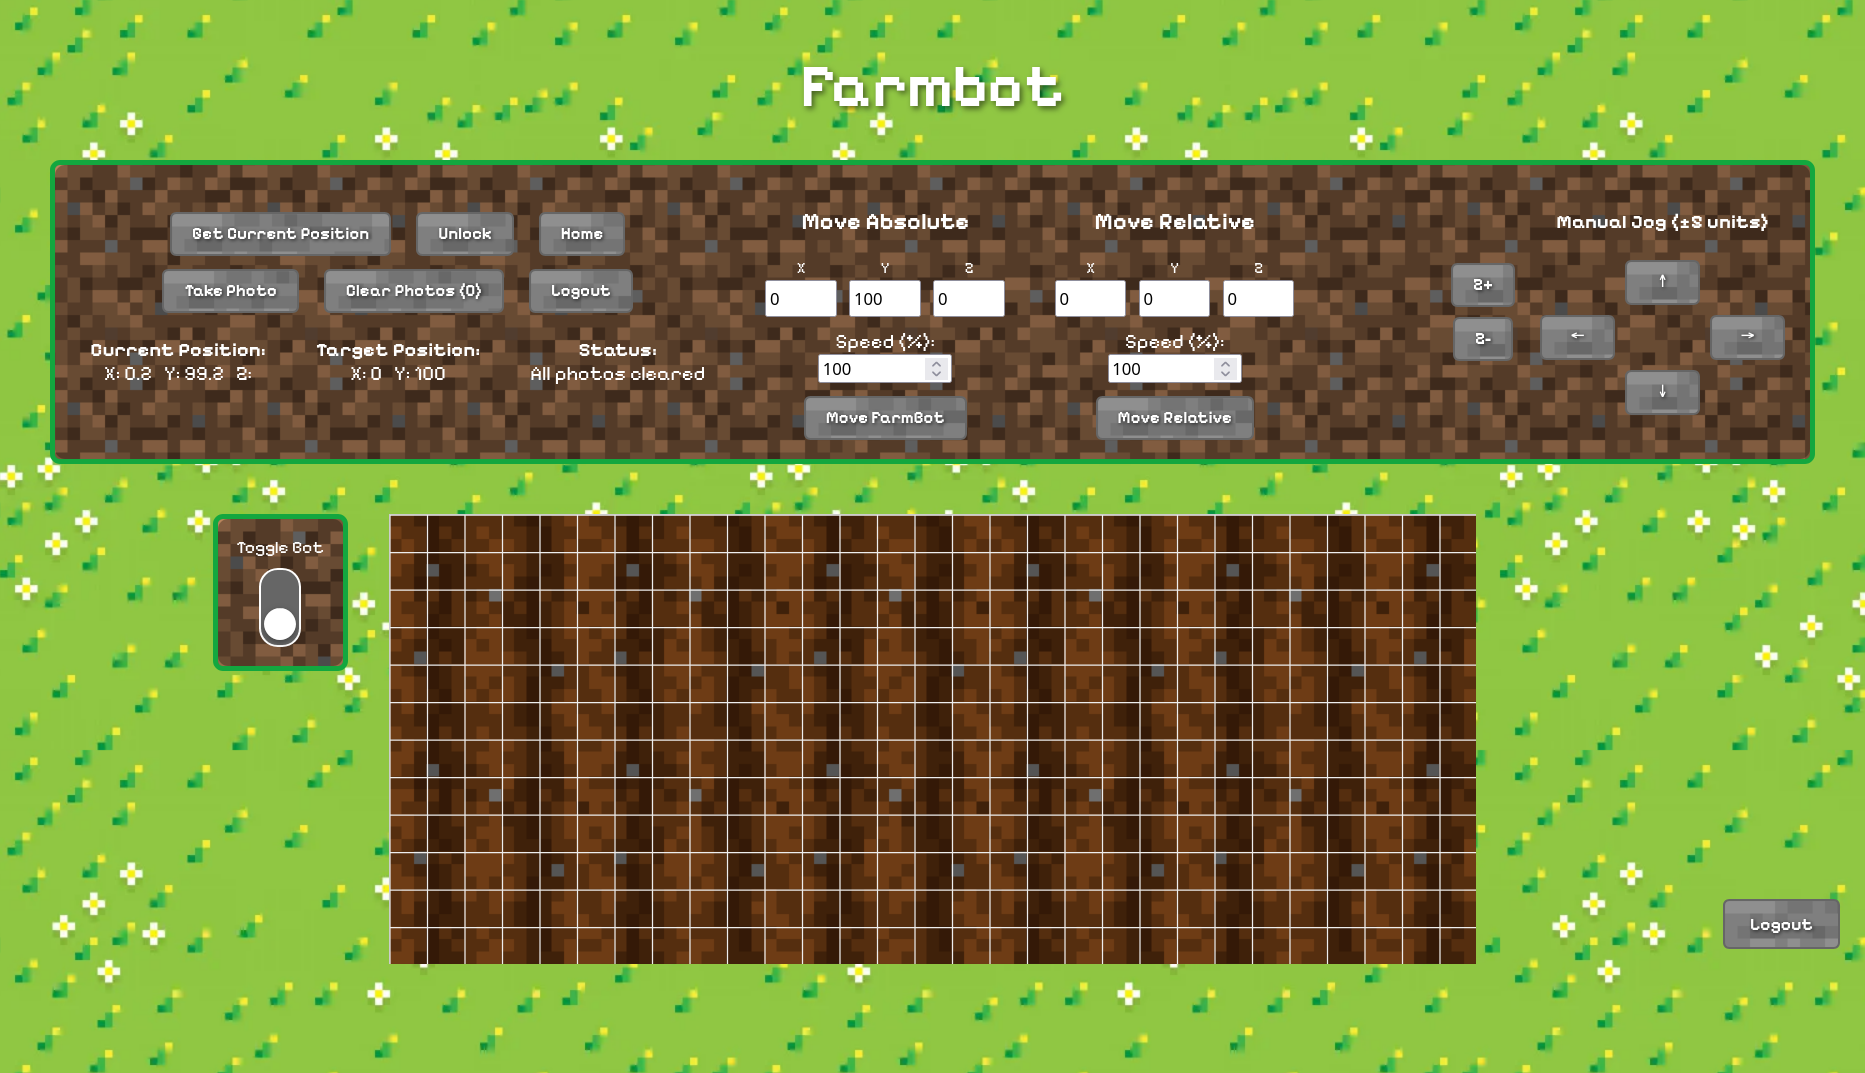
\includegraphics[width=0.8\textwidth]{img/clearing_photos.png}
    \caption{Clearing Photos}
    \label{fig:dashboard_clearing_photos}
\end{figure}

\newpage
\section{Hardware Architecture}

The FarmBot system's hardware architecture integrates multiple specialized components to ensure reliable and precise agricultural operations. The architecture emphasizes modularity, maintainability, and robust operation under various environmental conditions.

\subsection{Computational and Power Infrastructure}
The system's computational backbone consists of local real-time controllers managing immediate operations, edge compute nodes for local data processing, and ARM-based Linux computers for higher-level control. Power management features include solar-assist capabilities, carefully sized battery buffers, and comprehensive power monitoring systems, ensuring reliable operation with graceful degradation modes when needed.

\subsection{Maintenance and Support Systems}
To ensure long-term reliability, the hardware architecture includes comprehensive maintenance support features. These encompass diagnostic tools for system health monitoring, a well-documented spare parts management system, and extensive logging capabilities for tracking system performance and maintenance needs.
